\begin{frame}\begin{center}
    \LARGE\textbf{Introduction}
\end{center}\end{frame}
%-------------------------------------------------------------------------------
%-------------------------------------------------------------------------------
\begin{frame}
The \textbf{National Longitudinal Surveys (NLS)} are a set of surveys conducted by the US Department of Labor's Bureau of Labor Statistics, designed to gather information at multiple points in time on significant life events of several population samples of US citizens, especially their labor market activities.
\end{frame}
%-------------------------------------------------------------------------------
%-------------------------------------------------------------------------------
\begin{frame}
The \textbf{National Longitudinal Survey of Youth 1979 (NLSY79)} is a survey of men and women born in the years 1957-64. The NLSY79 is a nationally representative sample of 12,686 young men and women who were 14-22 years old when they were first surveyed in 1979. These individuals were interviewed annually through 1994 and are currently interviewed on a biennial basis.
\end{frame}
%-------------------------------------------------------------------------------
%-------------------------------------------------------------------------------
\begin{frame}\textbf{Topics}\vspace{0.3cm}
\begin{itemize}\setlength\itemsep{1em}
\item education, training, and achievement
\item employment
\item health
\item attitudes and expectations
\item cognitive and noncognitive scores
\item $\hdots$
\end{itemize}
\end{frame}
%-------------------------------------------------------------------------------
%-------------------------------------------------------------------------------
\begin{frame}\textbf{Subsamples}\vspace{0.3cm}
\begin{itemize}\setlength\itemsep{1em}
\item cross-sectional sample designed to be representative of the civilian segment of young people
\item supplemental sample designed to oversample civilian Hispanic, black, and economically disadvantaged non-black/non-Hispanic youth
\item military sample designed to represent the population who are enlisted in one of the four branches of the military
\end{itemize}
\end{frame}
%-------------------------------------------------------------------------------
%-------------------------------------------------------------------------------
\begin{frame}\begin{figure}[htp]\centering
\caption{Number of observations}
\scalebox{0.35}{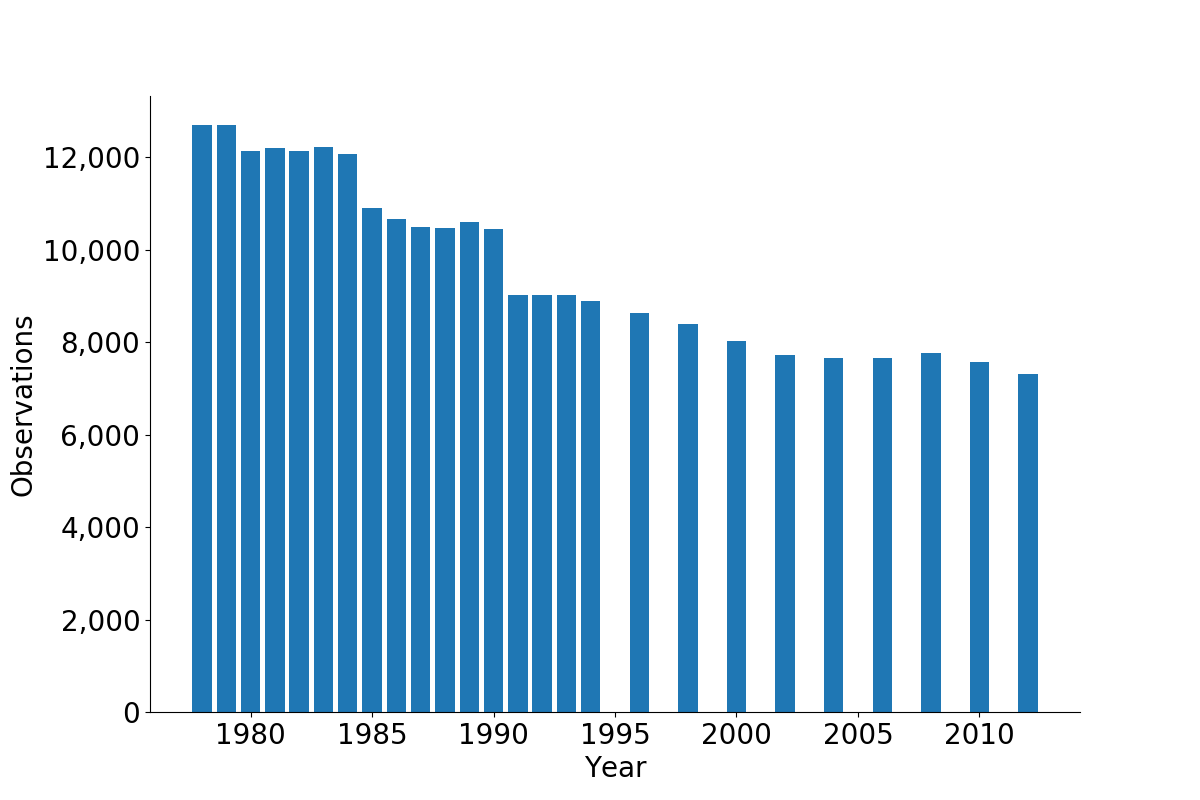
\includegraphics{fig-dataset-basic-observations}}
\end{figure}\end{frame}
%-------------------------------------------------------------------------------
%-------------------------------------------------------------------------------
\begin{frame}\begin{figure}[htp]\centering
\caption{Samples}
\scalebox{0.35}{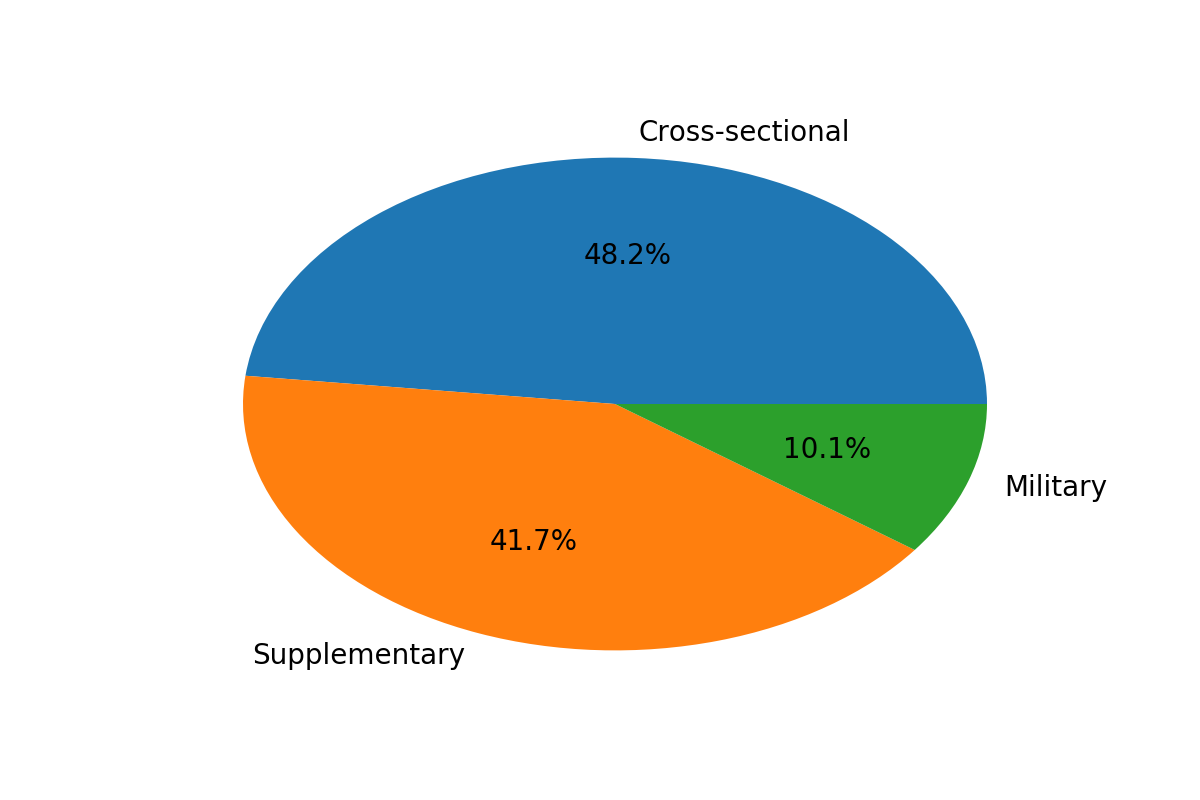
\includegraphics{fig-dataset-basic-samples}}
\end{figure}\end{frame}
%-------------------------------------------------------------------------------
%-------------------------------------------------------------------------------
\begin{frame}\begin{figure}[htp]\centering
\caption{Year of birth}
\scalebox{0.35}{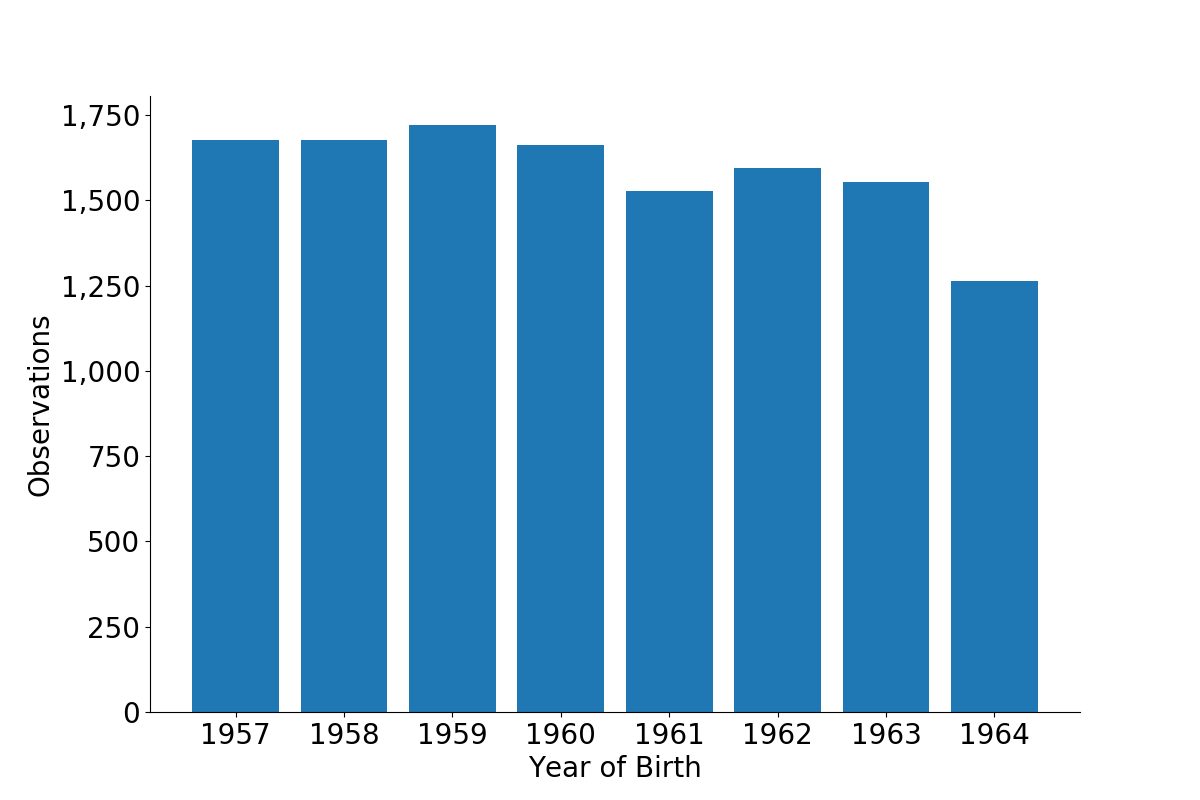
\includegraphics{fig-dataset-basic-birth}}
\end{figure}\end{frame}
%-------------------------------------------------------------------------------
%-------------------------------------------------------------------------------
\begin{frame}\begin{figure}[htp]\centering
\caption{Gender}
\scalebox{0.35}{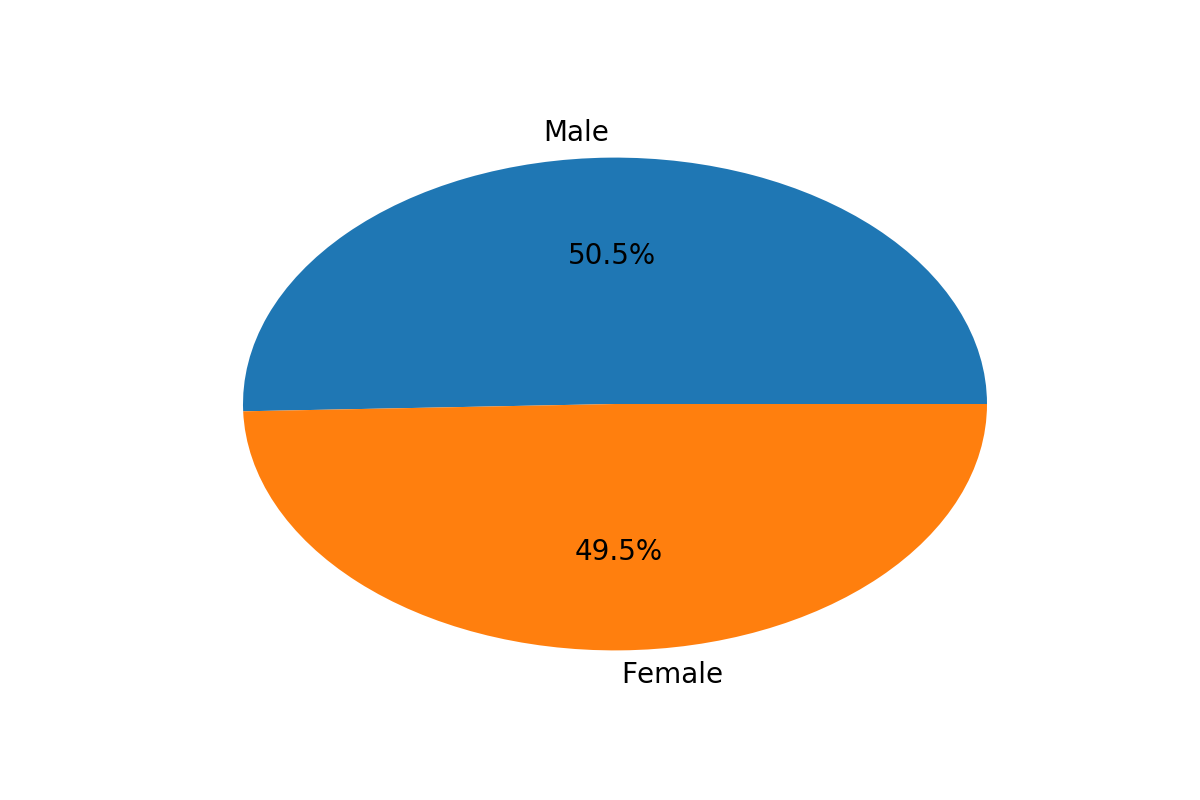
\includegraphics{fig-dataset-basic-gender}}
\end{figure}\end{frame}
%-------------------------------------------------------------------------------
%-------------------------------------------------------------------------------
\begin{frame}\begin{figure}[htp]\centering
\caption{Income quartile}
\scalebox{0.35}{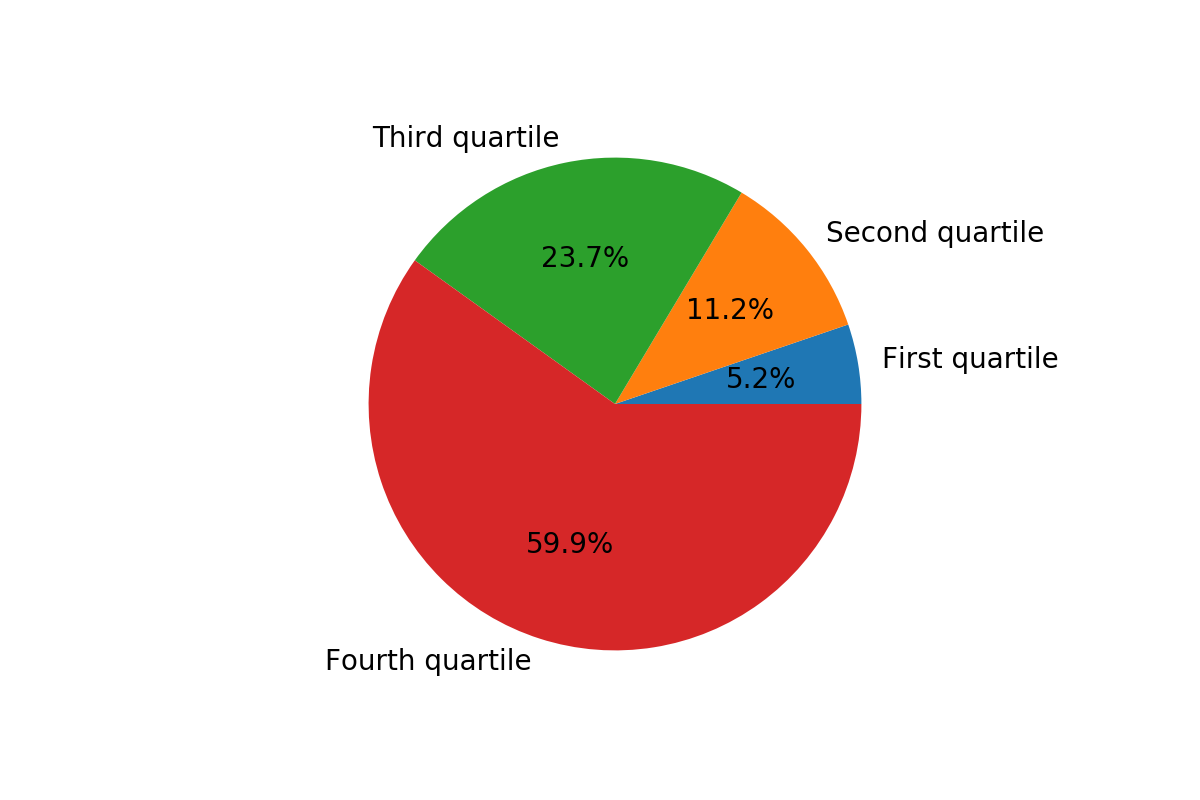
\includegraphics{fig-dataset-basic-income-quartile}}
\end{figure}\end{frame}
%-------------------------------------------------------------------------------
%-------------------------------------------------------------------------------
\begin{frame}\begin{figure}[htp]\centering
\caption{NLS Investigator I}
\scalebox{0.125}{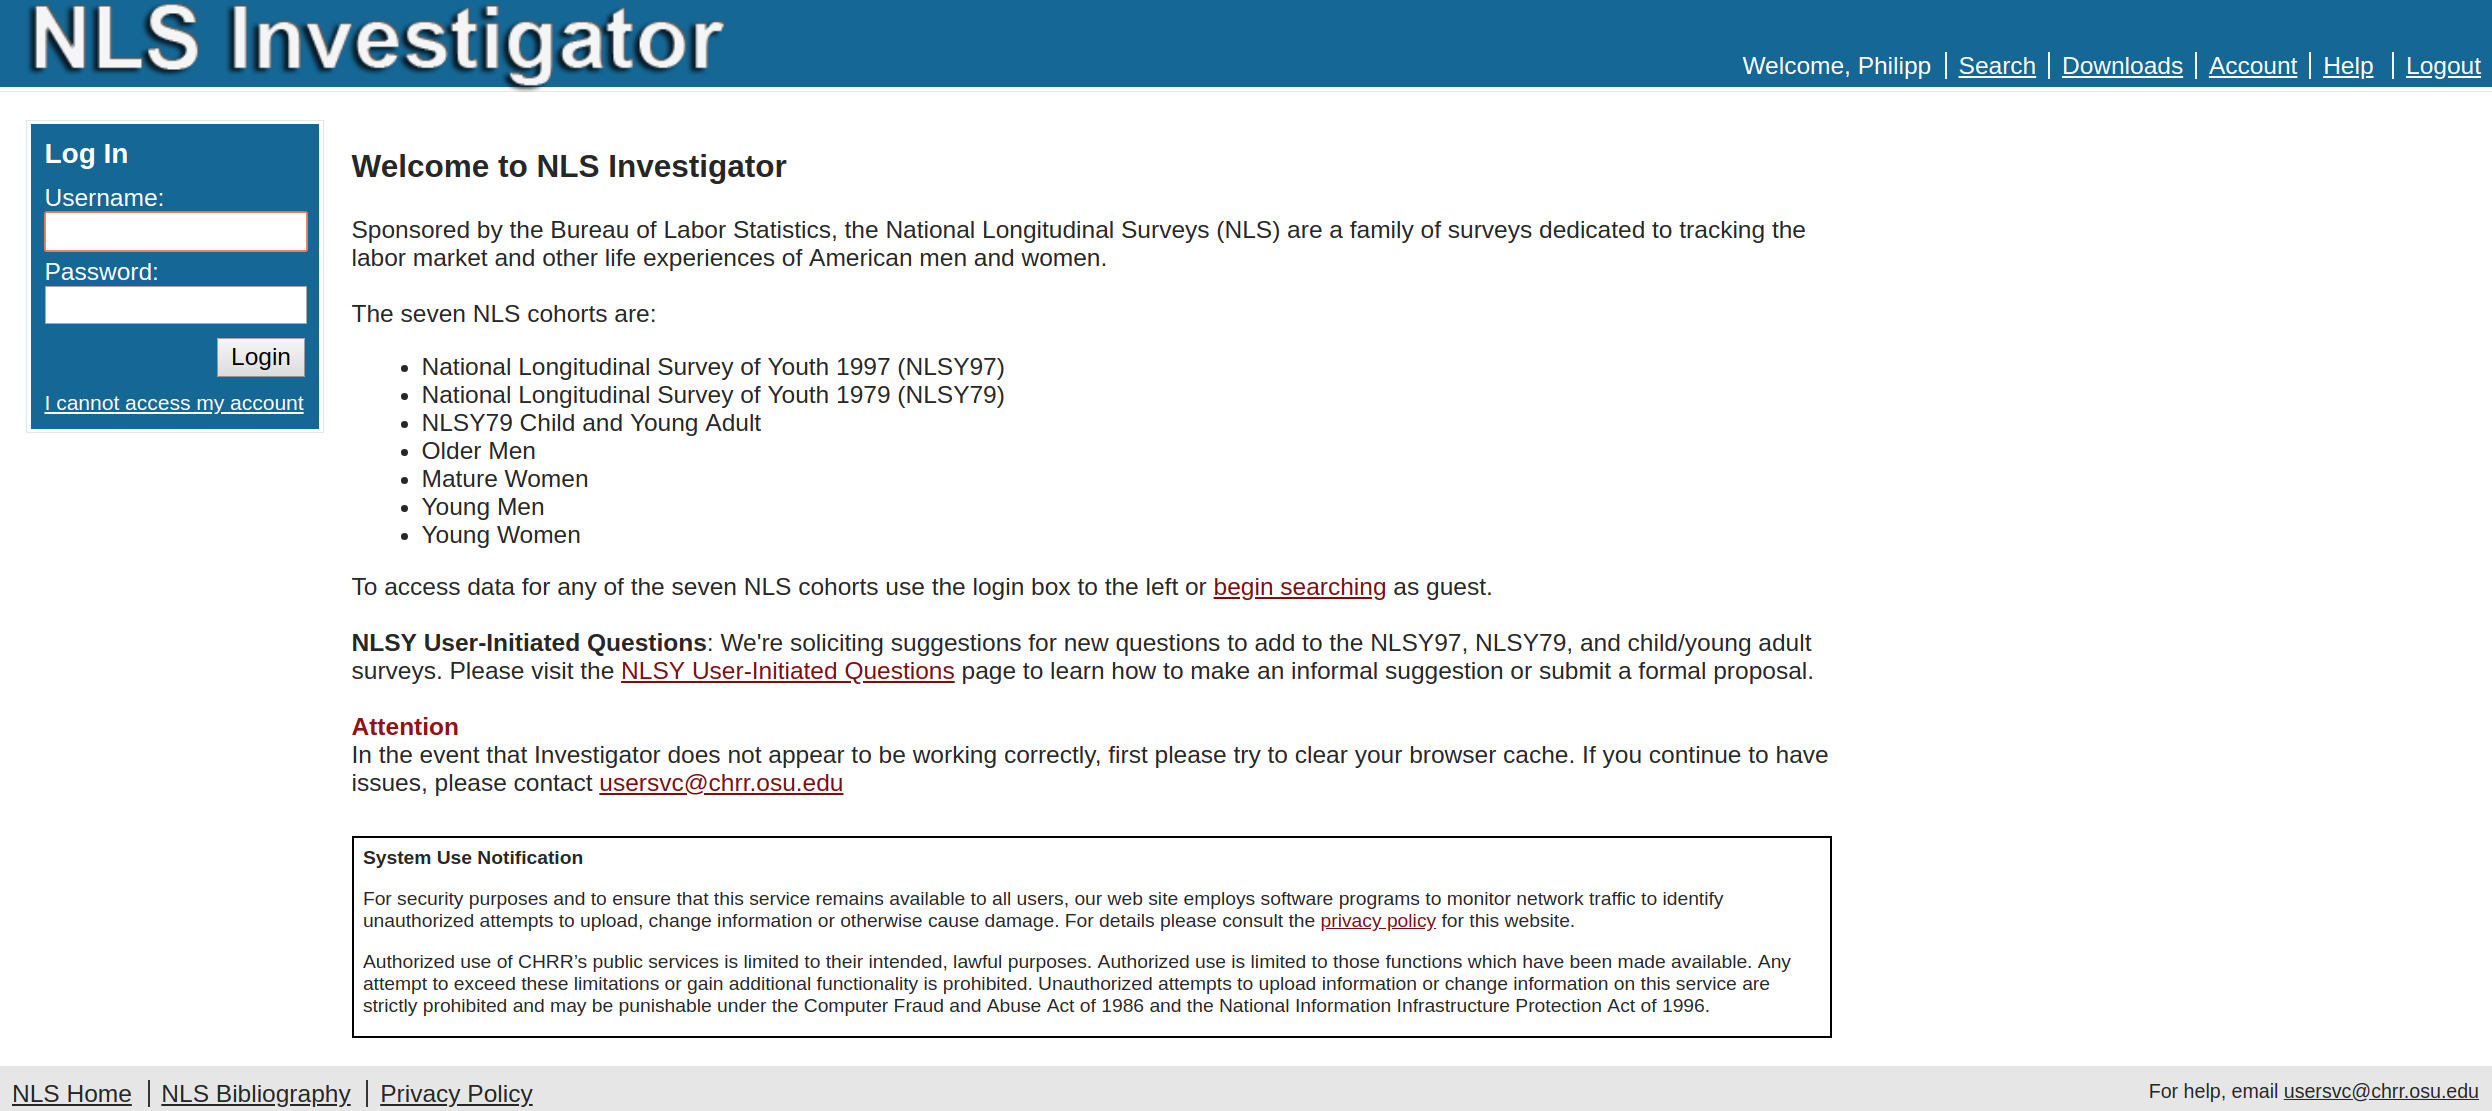
\includegraphics{fig-nls-investigator-1}}
\end{figure}\end{frame}
%-------------------------------------------------------------------------------
%-------------------------------------------------------------------------------
\begin{frame}\begin{figure}[htp]\centering
\caption{NLS Investigator II}
\scalebox{0.125}{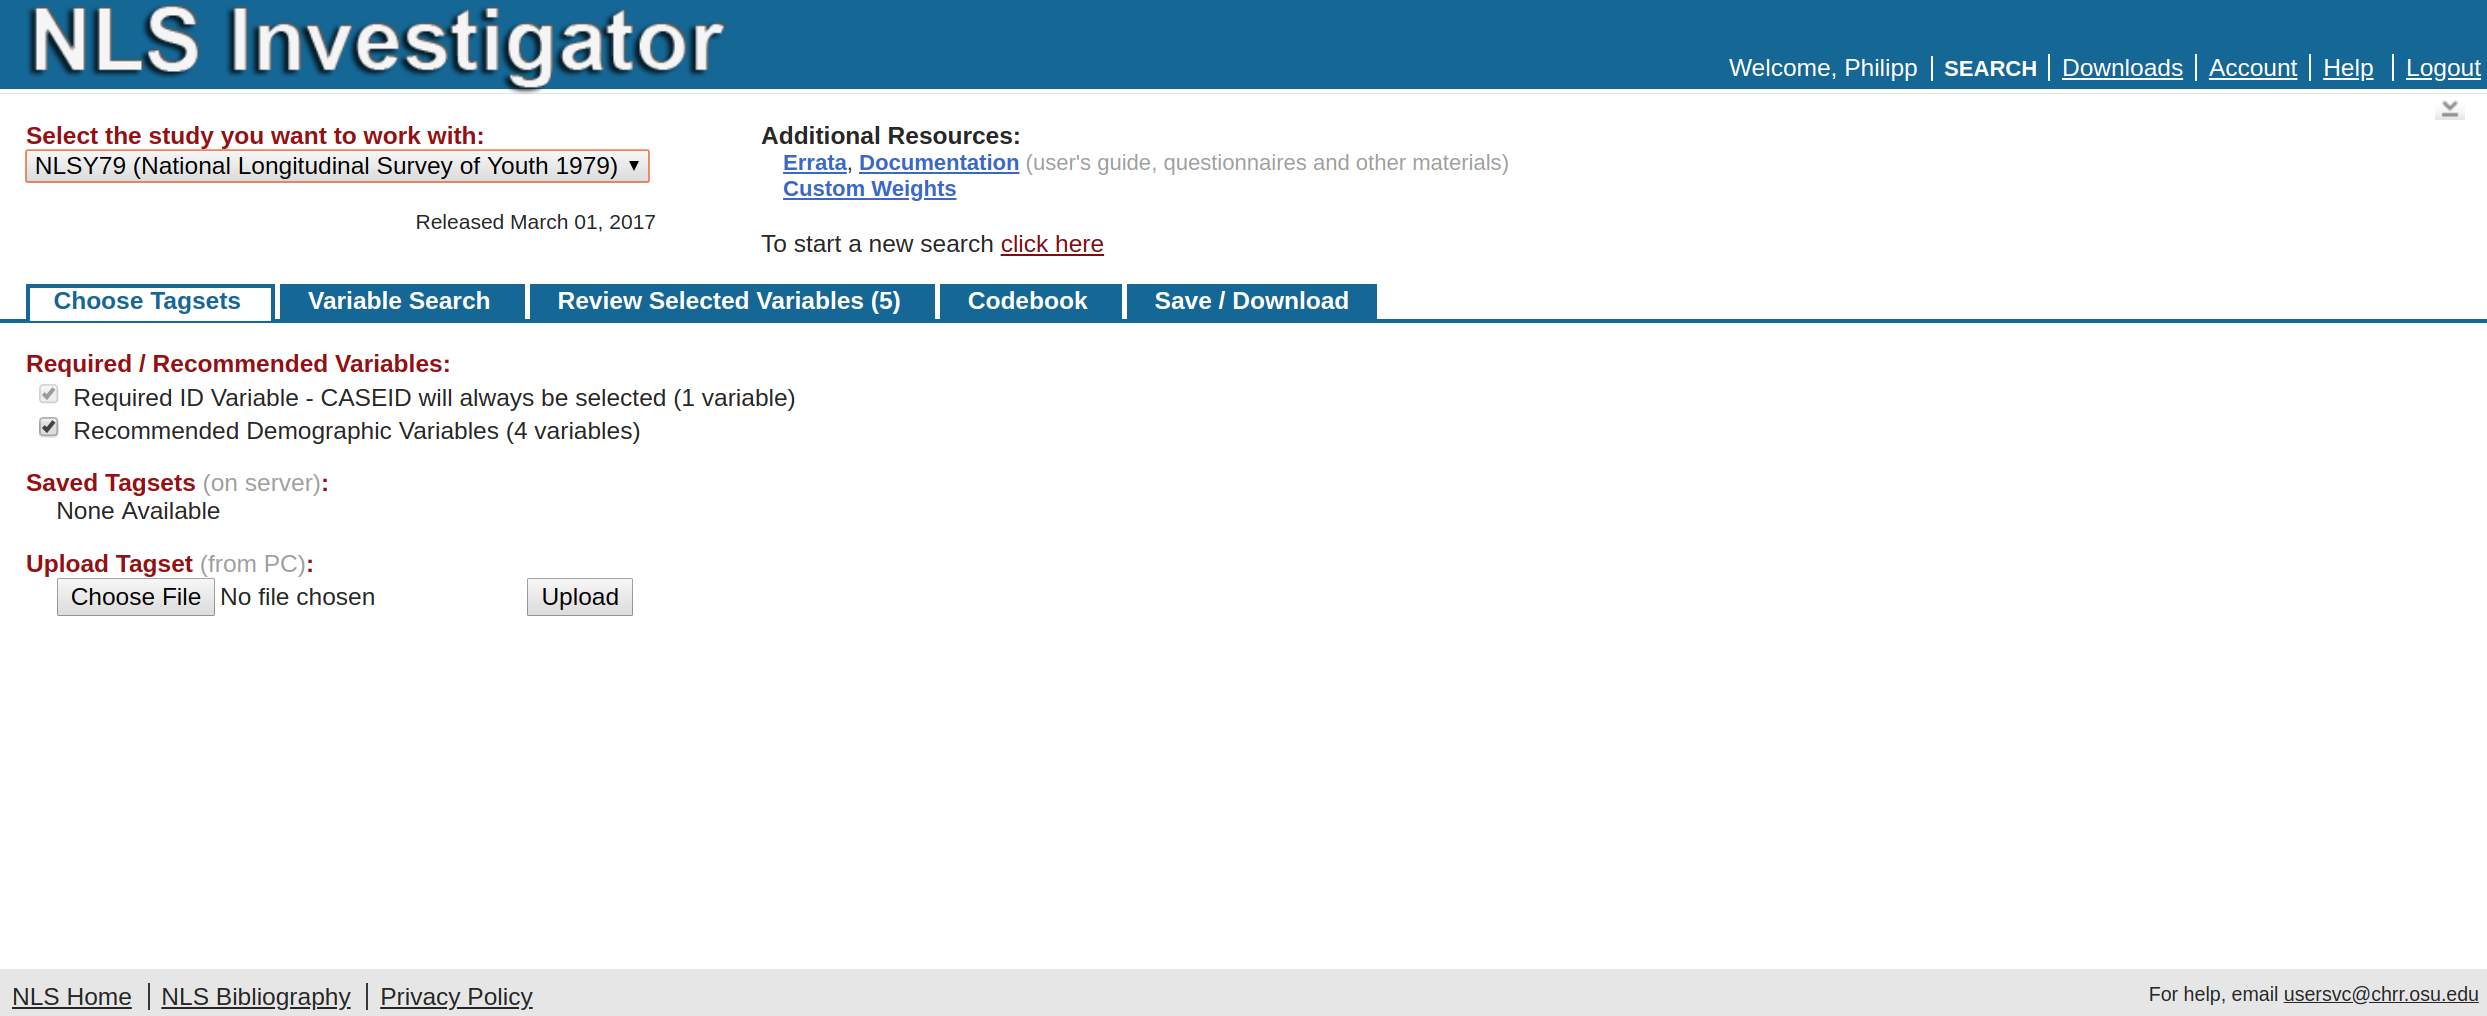
\includegraphics{fig-nls-investigator-2}}
\end{figure}\end{frame}
%-------------------------------------------------------------------------------
%-------------------------------------------------------------------------------
